\documentclass{sfuthesis}
\title{Speed and Accuracy Trade-off in Neural Network Models for Sequence Tagging}
\thesistype{Thesis}
\author{Xinxin Kou}
\previousdegrees{%
	B.Sc. (Hons.), Dalhousie University, 2015}
\degree{Master of Science}
\discipline{Computing Science}
\department{School of Computing Science}
\faculty{Faculty of Applied Sciences}
\copyrightyear{2017}
\semester{Fall 2017}
\date{12 September 2017}

\keywords{Natural Language Processing;}


%   PACKAGES AND CUSTOMIZATIONS  %%%%%%%%%%%%%%%%%%%%%%%%%%%%%%%%%%%%%%%%%%%%%%
%
%   Add any packages or custom commands you need for your thesis here.
%   You don't need to call the following packages, which are already called in
%   the sfuthesis class file:
%
%   - appendix
%   - etoolbox
%   - fontenc
%   - geometry
%   - lmodern
%   - nowidow
%   - setspace
%   - tocloft
%
%   If you call one of the above packages (or one of their dependencies) with
%   options, you may get a ''Option clash'' LaTeX error. If you get this error,
%   you can fix it by removing your copy of \usepackage and passing the options
%   you need by adding
%
%       \PassOptionsToPackage{<options>}{<package>}
%
%   before \documentclass{sfuthesis}.
%
\usepackage{natbib}
\usepackage{apalike}
\usepackage{amsmath,amssymb,amsthm}
\usepackage[pdfborder={0 0 0}]{hyperref}
\usepackage{graphicx}
\usepackage{caption}
%\usepackage[numbers]{natbib}
\usepackage{algorithm}
\usepackage{algpseudocode}
\usepackage{array}
\usepackage{multirow}
\usepackage{underscore}
\usepackage{pgfplots}
\pgfplotsset{width=10cm,compat=1.15}

\newcommand{\quotes}[1]{\textrm{``#1''}}

%   FRONTMATTER  %%%%%%%%%%%%%%%%%%%%%%%%%%%%%%%%%%%%%%%%%%%%%%%%%%%%%%%%%%%%%%
%
%   Title page, committee page, copyright declaration, abstract,
%   dedication, acknowledgements, table of contents, etc.
%

\begin{document}

\frontmatter
\maketitle{}

\begin{abstract}
Sequence Tagging including part of speech tagging and named entity recognition is an important task in NLP. The recurrent neural network models such as the Bidirectional LSTM models have produced impressive results on sequence tagging. In this work, we present simple and fast greedy sequence tagging system using variant feedforward neural network models. We also compare variant Bidirectional LSTM models on sequence tagging tasks. Besides the feedforward and the Bidirectional LSTM models, we present two multitask models based on the Mention2Vec Model: a model using Byte Pair Encoding to segment words for part-of-speech tagging and a model separating boundary and tag prediction for named entity recognition. We carefully design the experiments to show the relationship between speed and accuracy when using different models. Our experiment results show that the greedy sequence tagging system with a feedforward network can achieve comparable accuracy and faster speed than the system using the recurrent models, and the multitasking model for named entity recognition is competitive with the fully structured BiLSTM model while being more scalable.

\end{abstract}


\begin{acknowledgements} % optional

I would like to express my profound sense of gratitude to my supervisor Dr.\ Anoop Sarkar for introducing me to this research
topic and providing his continuous support and valuable guidance throughout my graduate study. I can not imagine having a better advisor and mentor. In addition, I would like to express my sincere appreciation to Dr. Fred Popowich for his useful advice and feedback on this work.




\end{acknowledgements}

\addtoToC{Table of Contents}\tableofcontents\clearpage
\addtoToC{List of Tables}\listoftables\clearpage
\addtoToC{List of Figures}\listoffigures





%   MAIN MATTER  %%%%%%%%%%%%%%%%%%%%%%%%%%%%%%%%%%%%%%%%%%%%%%%%%%%%%%%%%%%%%%
%
%   Start writing your thesis --- or start \include ing chapters --- here.
%

\mainmatter%

\chapter{Introduction}

In this chapter, we first describe the sequence tagging tasks and introduce the motivation of this thesis. Then, we summarize our major contributions and describe the structure of the thesis.

\section{Sequence Tagging Task}

In this section, we briefly introduce two sequence tagging tasks on which we will benchmark different neural network models in this thesis. The experimental data are summarized in Table \ref{table:my-dataset}, while performance using existing models are reported in Table \ref{table:my-performance}.

\subsection{Part-of-Speech Tagging (POS)}
Part-of-Speech Tagging (POS) assigns each word with a unique tag that indicates its syntactic role, such as noun, adverb, verb \dots as illustrated in Figure \ref{fig:pos-ex}. 

Most POS systems are evaluated on the English Penn TreeBank data set(~\citeauthor{marcus1993building}, ~\citeyear{marcus1993building}), which contains 45 part-of-speech tags. The standard split uses section 1-18 of the Treebank for training, section 19-21 for tuning, and section 22-24 for testing (~\citeauthor{toutanova2003feature}, ~\citeyear{toutanova2003feature}). A lot of existing models are linear statistical models: Hidden Markov Models(HMM) obtains 96.46\% per word accuracy (~\citeauthor{mccallum2000maximum}, ~\citeyear{mccallum2000maximum}); the averaged perception discriminative model obtains 97.11\% per word accuracy (~\citeauthor{collins2002discriminative}, ~\citeyear{collins2002discriminative}). More recently, neural network models pushed up the state-of-the-art scores. The BI-LSTM-CRF model by \cite{huang2015bidirectional} reaches 97.55\% per word accuracy, and the compositional character-to-word LSTM model of \cite{ling2015finding} reaches 97.78\% per word accuracy. 

In this thesis, we conduct the POS experiments on the English Penn TreeBank data set and the OntoNotes data set (~\citeauthor{hovy2006ontonotes}, ~\citeyear{hovy2006ontonotes}).



\subsection{Named Entity Recognition (NER)}

Named Entity Recognition (NER) is a sub-problem of
information extraction which identifies expressions
that refer to peoples, places, organizations and others. A popular convention is to use the "IOB" label scheme (Inside, Outside, Beginning): if the token is the beginning of a named entity tag, it is labeled as B-label; if the token is inside a named entity tag but not the first one, it is labeled as I-label; if the token is outside the named entity tag, it is labeled as O. An example of NER is shown in Figure \ref{fig:ner-ex}.

The shared task of CoNLL2003 (~\citeauthor{tjong2003introduction}, ~\citeyear{tjong2003introduction}) of NER contains 4 types of named entities: locations (LOC), persons (PER), organizations (ORG), and miscellaneous (MISC).
The best system presented at the NER CoNLL 2003 challenge by \cite{florian2003named} obtains 88.76 F1 score. The Bidirectional LSTM CRF model by \cite{huang2015bidirectional} reaches 88.83 F1 score. Both of these models use a lot of external features along with a large gazetteer. \cite{lample2016neural} proposed two NER models with no external features or gazeteer: the first one makes structured prediction using Bidirectional LSTM, character embeddings and CRF; and the second one uses a Shift-Reduce framework with Stack-LSTM. The first model achieves the state-of-the-art result while the second one preforms slightly worse. 


In this thesis, we conduct the NER experiments on the CoNLL2003 data set and OntoNotes data set which contains 18 types of named entities. 


%\textbf{GLoVE} It's been shown that using pretrained word embeddings leads to significant performance improvement on sequence tagging (~\citeauthor{collobert2011natural}, ~\citeyear{collobert2011natural}; ~\citeauthor{lample2016neural}, ~\citeyear{lample2016neural}). In the experiments of this thesis, we use the GloVe vector representations for words (~\citeauthor{pennington2014glove}, ~\citeyear{pennington2014glove}), which has 40K vocabulary size and each word corresponds to a 100-dimensional embedding vector.

\begin{table}[]
\centering
\caption{Number of sentences, words and labels in each training, validation and test data set}
\label{table:my-dataset}
\begin{tabular}{|c|c|c|c|c|} \hline
      & Training  & Validation  & Test  & labels  \\ \hline
Penn Treebank   &39831(950011) &1699(40068) &2415(56671) &45\\\hline
CoNLL2003   &14987(204567) &3466(51578) &3684(46666) &9     \\\hline
OntoNotes   & & & &18     \\\hline
\end{tabular}
\end{table}


\begin{table}[]
\centering
\caption{Performance of different POS and NER systems. Performance is reported in per-word accuracy for POS, and F1 score for NER. }
\label{table:my-performance}
\begin{tabular}{cclcc}
POS Systems       & Accuracy &  & NER Systems           & F1
\\ \cline{1-2} \cline{4-5} 
\text{\cite{mccallum2000maximum}} & 96.46\%                      &  & \text{\cite{florian2003named}}                 & 88.76                  \\
\text{\cite{collins2002discriminative}}    & 97.11\%                      &  & \text{\cite{huang2015bidirectional}}           & 88.83                  \\
\text{\cite{huang2015bidirectional}}       & 97.55\%                      &  & \text{\cite{lample2016neural}} with CRF        & 90.94                  \\
\text{\cite{ling2015finding}}              & 97.78\%                      &  & \text{\cite{lample2016neural}} with Stack LSTM & 90.33                 
\end{tabular}
\end{table}

\begin{figure}
  \centering
  \includegraphics[scale=0.4]{pos-ex.png}
 \caption{An example of POS}
  \label{fig:pos-ex}
\end{figure}

\begin{figure}
  \centering
  \includegraphics[scale=0.5]{ner-ex.png}
 \caption{An example of NER}
  \label{fig:ner-ex}
\end{figure}

\section{Motivation}

Bidirectional Long Short-Term Memory (BiLSTM) (~\citeauthor{Hochreiter97longshort-term}, ~\citeyear{Hochreiter97longshort-term}; ~\citeauthor{graves2005framewise}, ~\citeyear{graves2005framewise}) networks have obtained impressive results in many NLP tasks. BiLSTM networks are popular models for solving sequence tagging problems for the reason that they can maintain information based on the past and future features in the input sequence. Based on the existing work, the state-of-the-art results on POS and NER can be obtained by using the BiLSTM model with Character Embeddings and CRF (~\citeauthor{ling2015finding}~\citeyear{ling2015finding}; ~\citeauthor{lample2016neural}, ~\citeyear{lample2016neural}). Some work has shown that using feedforward neural network can achieve comparable results or better accuracy than models using BiLSTMS in tasks such as POS and Dependency Parsing. One approach is to employ a greedy transition system with a feedforward network to make independent classification decision on each word. However, the greedy system is limiting when there are strong correlations between output labels. NER is one of such tasks which have grammar constrains on the output label sequence. For example, the "I-PER" tag cannot follow the "B-LOC" tag in NER. In order to take into account the strong dependencies between output labels, a conditional random field layer (CRF) (~\citeauthor{lafferty2001conditional}, ~\citeyear{lafferty2001conditional}) can be added to model the output label sequence jointly. Since the CRF models focus on the sentence level, they take more time in decoding the sequence. We are interested in the speed-accuracy trade-off of different models in this thesis. Therefore, we re-implement variants of feedforward models and BiLSTM models in Tensorflow and systematically compare the performance and decoding speed of them on sequence tagging tasks.

Since the named entity tags in NER often span multiple tokens, most neural architectures for NER predict the boundary and the type of entities together using the the IOB label scheme. Mention2Vec (~\citeauthor{stratos2016mention2vec}, ~\citeyear{stratos2016mention2vec}) is proposed to address the natural segment-level representation in NER by separating the NER task into boundary detection (IOB) and type prediction (PER, LOC, etc.). While Mention2Vec employs two BiLSTMs for each sub-task, we replace the the BiLSTMs for boundary detection with the feedforward network with CRF in order to accelerate the classification and capture the dependencies of boundary tags. This new model is denoted as Feedforward-Mention2Vec in this thesis.

Inspired by the work using Byte Pair Encoding (BPE) (~\citeauthor{gage1994new}, ~\citeyear{gage1994new}) to deal with rare words in sentences(~\citeauthor{sennrich2015neural}, ~\citeyear{sennrich2015neural}), we come up with a new model combining BPE and Feedforward-Mention2Vec for POS, which is denoted as BPE-Mention2Vec. We use BPE to segment the input words in the hope of capturing the orthographic evidence of the words without using spelling features (like prefixes and suffixes) or character embeddings. After the word segmentation, POS becomes a NER-like task. Since the boundaries of the output labels are known in POS, we can use Feedforward-Mention2Vec for type prediction only.

\section{Contribution}
The three main contributions of this thesis are:

\begin{enumerate}

\item We implement a greedy tagging system with two feedforward network architectures. The first architecture takes context word features, spelling features, and history tag features as input. The second architecture uses context word features and CRF to model the output sequences. There are few work measuring the decoding time using feedforward networks on sequence tagging. We conduct the experiments on NER and POS, and then record the performance and decoding speed on different data sets. To show the robustness of the feedforward network, we also conduct the experiments using a feedforward network with only word features. We benchmark different feedforward models and provide analysis on the results. 

\item We implement the fully structured Bidirectional LSTM model, which uses character embeddings and CRF. There is few work comparing the Bidirectional LSTM model with different configurations in terms of decoding speed, such as if the model is using character embedding and if the model is using CRF. We conduct the experiments using the Bidirectional LSTM model with different configurations on POS and NER. We benchmark the performance and decoding speed of different Bidirectional LSTM networks. 

\item We introduce two new neural architectures based on the Mention2Vec model: Feedforward-Mention2Vec for NER and BPE-Mention2Vec for POS. The original Mention2Vec model is designed for NER using BiLSTMs to predict named entity boundaries and types separately. In Feedforward-Mention2Vec, we use the feedforward network with CRF in our new models to predict the named entity boundaries. We also adapt the model for POS by combining BPE. BPE is used for word segmentation so that it turns POS to a NER-like task. In the BPE-Mention2Vec model for POS, we first use BPE to segment the input words, and then we use a Bidirectional LSTM to predict the types for word spans. We benchmark these two multitasking models with the feedforward models and the Bidirectional LSTM models in terms of performance and speed. Our experiments show that the feedforward model produces comparable results while being significantly faster on both NER and POS. Our experiments also show the Feedforward-Mention2Vec model achieves competitive score and decode faster than the Bidirectional LSTM model on NER.

\end{enumerate}


\section{Overview}
The thesis is organized as follows:

In \textbf{Chapter 2}  we present the feedforward network model with three different configurations: feedforward network with only word features; feedforward network with spelling feature and history features; feedforward network with CRF. We explain the training and decoding process using the feedforward models, demonstrate the experiment design, and benchmark the performance and decoding time of the feedforward models with different configurations.

In \textbf{Chapter 3} we present variants Bidirectional LSTM Network models: Bidirectional LSTM with only word features (BiLSTM), Bidirectional LSTM with character embeddings (BiLSTM-Char), and fully structured BiLSTM (Bidirectional LSTM with character embeddings and CRF) (BiLSTM-Char-CRF). We explain the training and decoding process using the BiLSTM models, demonstrate the experiment design, and benchmark the performance and decoding time of the different Bidirectional LSTM Network models.

In \textbf{Chapter 4} we present two new multitask models based on the Mention2Vec Model: the Feedforward-Mention2Vec for NER and BPE-Mention2Vec for POS. We explain the architecture of these two models and benchmark them with the feedforward models and the BiLSTM models in terms of performance and speed.

In \textbf{Chapter 5} we summarize and discuss the experimental results from the previous chapters. We analyze the trade-off between performance and speed of different neural network models.


\chapter{Feedforward Neural Network Models}

In this chapter, we describe two feedforward network models: Feedforward-history and Feedforward-crf. Throught carefully designed experiments, we show the performance and decoding speed of different feedforward models.

\section{Network Architecture}
Inspired by the greedy parser system by ~\cite{chen2014fast}, we present a similar greedy transition system for sequence tagging in this section. The greedy parser system employs a basic arc-standard system (~\citeauthor{nivre2004deterministic}, ~\citeyear{nivre2004deterministic}), which consists of three types of transitions(LEFT-ARC, RIGHT-ARC, and SHIFT), a stack, and a buffer. While the greedy parser system has three types of actions, the sequence tagging system only has SHIFT action which predicts the tag of the current word in the buffer and shifts the word to the stack. 

In the greedy sequence tagging system, we assume that the word to be labeled depends mainly on its neighbors instead of the whole sentence. There are two ways to make use of neighbor label information: the first one is to use the previous predicted labels as input features the model feeds into the feedforward network layer; the second one is to use CRF on sentence level output labels instead of individual labels. Two architectures using these two methods respectively are introduced in this section. The Feedforward Network with History model makes use of the first method to incorporate the history labels as features, and the Feedforward Network with CRF model adds a CRF layer on the output label sequence. These two architectures are similar with the window approach proposed in ~\cite{collobert2011natural}.



\subsection{Feedforward Neural Network with History}

Figure \ref{fig:greedypos} illustrates the architecture of the POS tagging system using the Feedforward Neural Network with History (Feedforward-History) model. We describe the Feedforward-History model in detail here. Since the current word depends on its neighbors in the greedy sequence tagging system, we use a fixed size window around the current word to generate features. In order to generate features for the words at the beginning and at the end of the sentence, we add a special “PADDING” word $window size/2$ times at the beginning and the end. To generate dense word features, we represent each word in the input sentence as a $d$-dimensional embedding vector $e_{wi}$. Meanwhile, we have a full vocabulary embedding vector dictionary $E_{w}$. Given a word $w_{i}$, we look up its embedding vector in $E_{w}$. Other spelling features of a word might help predict the label of the word as well, such as upper and lower case features, prefix and suffix features. Each spelling feature of a word $w_{i}$ is associate with a $d$-dimensional embedding vector $e_{si}$ and a embedding vector dictionary $E_{s}$. Besides word features and spelling features, we incorporate the output label features in this model. Since the greedy sequence tagging system labels word by word in a sentence, we can only use the previous labels as input features for predicting the labels for the current word. The input layer is obtained by concatenating the word feature vectors, spelling feature vectors, and history label feature vectors. Generating features for sequence tagging are expensive: selecting useful features is an empirical process based trial and error, and computing features vectors needs to concatenate feature strings and search them in a huge lookup table. We try to use features as little as possible to cut the time of feature generation while keeping the model accurate. In the model implementation, we extract the word and spelling features on a window size of 8 centered on the current focus word. We extract the following spelling features of each word: whether start with a capital letter; whether has all capital letters; whether has a mix of letters and digits; whether has punctuation; letter prefixes and suffices of length 2 and 3. We also extract the history label features on the previous 4 predicted labels. In order to build a simple and fast network model, we only use one hidden layer in this model. The input layer is mapped to a hidden layer through a Relu activation function:

\begin{equation}
H=Relu\left(\left( W_{1}^{w}x^{w}+W_{1}^{s}x^{s}+W_{1}^{l}x^{l}\right)\right),
\end{equation}

where $x^{w}$ represents the word input features, $x^{s}$ represents the spelling input features, $x^{l}$ represents history label input features, $W_{1}$ is the weight parameter for the hidden layer. Label probability distribution is modeled by a softmax layer:

\begin{equation}
p=softmax\left(W_{2}H+b\right),
\end{equation}

where $W_{2}$ is the weight parameter for the softmax layer and b is the bias.

The network is trained by minimized a negative log likelihood over the training data. The embedding vectors are trainable inputs for the network. We denote all trainable parameters as $\theta$.

For an input sentence:

\begin{center}
$X=\left( w_{1},w_{2},\ldots w_{n}\right)$, 
\end{center}

and a sequence predictions

\begin{center}
$Y=\left( y_{1},y_{2},\ldots y_{n}\right)$,
\end{center}

$p\left( y_{i}|x_{i}\right)$ is the conditional probability over $y_{i}$.

\subsection{Feedforward Neural Network with CRF}
\label{Feedforward-CRF}
Feedforward Network with CRF (Feedforward-CRF) shares the same architecture with Feedforward-History except using CRF on sentence level instead of making independent decisions for each word. Feedforward-History can perform well on some sequence tagging tasks in which output labels do not have strong correlations, such as POS. Some tasks have grammar constrains on the output labels so that the labels are dependent in each sentences, such as NER. While Feedforward-History fails to take into account the grammar constrains, Feedforward-CRF model the output decisions in a sentence jointly. We describe how to apply CRF to model the sequence in detail here. Since the first part of the architecture is the same with Feedforward-History, we use the same notations.

For a sequence of output predictions:

\begin{center}
$Y=\left( y_{1},y_{2},\ldots y_{n}\right)$
\end{center}

The score of the output sequence is:

\begin{equation}
S\left( X|Y\right)=\sum _{i}^{n}T_{i,i+1}+\sum _{i}^{n}P_{i}
\end{equation}

where $T$ is a matrix of transition scores such that $T_{i,j}$ represents the score of a transition from the label $i$ to label $j$.

During training, we score every possible output sequences, and minimize the negative log likelihood over the training sentences. With the transition matrix $T$, we can decode the tag sequences of the test data using dynamic programming.



\begin{figure}
  \centering
  \includegraphics[scale=0.6]{greedypos.png}
 \caption{The architecture of the POS tagging system using a feedforward neural network.}
  \label{fig:greedypos}
\end{figure}


\section{Experiments and Results}
To evaluate the feedforward models, we run our models (Feedforward-history, Feedforward-CRF) on POS and NER, and we report the performance and decoding speed of the models. The performance of POS is measured by the per word accuracy, and the performance of NER is measured by the F1 score. The speed is measured by the average number of words decoded per second. We also want to show the robustness of the greedy system with the feedforward network model, so we run experiments using the feedforward model with only word features, denoted as Feedforward-word in this thesis. 

In the POS experiments, we train the models using the Penn Treebank training data and development data. Then, we decode the Penn Treebank test data with trained models and record the per word accuracy and decoding time. In the NER experiments, we train the models uisng the Conll2003 training data and development data. Then we decode the test data with the trained models, and record the F1 score and decoding time. The details of the data sets are shown in Table \ref{table:my-dataset}.

 
We implement the models using the Tensorflow library, and use the GLoVE pre-trained word embedding where each word corresponds to a 100-dimensional embedding vector. We tuned the hyper-parameters for training. Specifically we use Adam (~\citeauthor{kingma2014adam}, ~\citeyear{kingma2014adam}) for stochastic optimization, set the learning rate to be 0.001, and the hidden layer to be 128. We have the batch implementation which processes multiple sentences at the same time, and we set the batch size to be 32 in the experiments. We run all the experiments in this thesis on a GeForce GTX 1080 GPU. 

Table \ref{table:ff-table1} and Table \ref{table:ff-tabel2} demonstrate our final benchmark result of three feedforward models on POS and NER. Figure \ref{fig:ff} illustrates the performance of the three models in a bar chart. In POS, Feedforward-word is 1.39\% less accurate then Feedforward-history. In NER, the F1 score of Feedforward-word is 2.42 lower than Feedforward-history. Since only using word features does not decrease the POS performance too much, we can conclude that greedy sequence tagging system with the feedforward model is robust with respect to spelling features on POS. The spelling features are more helpful in NER. In both POS and NER, Feedforward-CRF has better performance than Feedforward-history, but it improve the performance more on NER because of the dependencies between the sequence labels in NER.

It's obvious that Feedforward-word has the fastest decoding speed because it doesn't use any extra features. Feedforward-crf is slower than the Feedforward-history since the CRF model compute the score of every possible output sequences.

\begin{table}[]
\centering
\caption{Feedforward Neural Network Models Accuracy and F-Score Comparison}
\label{table:ff-table1}
\begin{tabular}{|c|c|c|}
\hline
Model         & POS (Accuracy)  & NER (F-Score)       \\ \hline
Feedforward-word    & 95.89          &   84.12     \\ \hline
Feedforward-history & 97.28     & 86.54        \\ \hline
Feedforward-CRF     & 97.30          &   87.85     \\ \hline
\end{tabular}
\end{table}

\begin{table}[]
\centering
\caption{Feedforward Neural Network Models Speed Comparison}
\label{table:ff-tabel2}
\begin{tabular}{|c|c|c|}
\hline
Model       & POS  (sentences, words/sec)  & NER  (sentences, words/sec)      \\ \hline
Feedforward-word    & 504(11831)     & 780(9886)    \\ \hline
Feedforward-history & 432(10137)     & 675(8562)     \\ \hline
Feedforward-CRF    & 376(8827)     & 610(7738)     \\ \hline
\end{tabular}
\end{table}

\begin{figure}
  \centering
  \includegraphics[scale=0.6]{ff.png}
 \caption{Feedforward Neural Network Models results}
  \label{fig:ff}
\end{figure}



\chapter{Bidirectional Long Short Term Memory Network Models}
In this chapter, we first describe the fully structured Bidirectional LSTM network (BiLSTM-Char-CRF). Then, we show the performance and decoding speed of the BiLSTM with different configurations.

\section{Model Description}
Feedforward neural networks can not directly use the previous data and future data to predict the current output, which is a drawback of applying feedforward network models on sequence tagging. 
Recurrent neural networks (RNNs) are networks with loops in them which allows data to persist. LSTMs are special RNNs with Long Short Term memory cells (~\citeauthor{graves2005framewise}, ~\citeyear{graves2005framewise}) illustrated in Figure \ref{fig:lstmcell}. However, RNNs is biased towards the most recent data in practice. The LSTM network is designed to address this issue: it learns long dependencies in a sequence with help of the structure of gates. The gates control how much of the input is given to the LSTM cell, and how much of the previous information to forget. 

\begin{figure}
  \centering
  \includegraphics[scale=0.6]{lstmcell.png}
 \caption{The architecture of a LSTM cell}
  \label{fig:lstmcell}
\end{figure}

Given a sentence with n words, LSTM computes a forward representation $\overrightarrow {h_{i}}$ for word i. In general, computing a backward representation $\overleftarrow {h_{i}}$ would be useful for sequence tagging. Computing both forward and backward hidden embeddings can be achieved by Bidirectional LSTMs (BiLSTMs). Figure \ref{fig:bilstm} illustrates the architecture of the POS tagging system using the BiLSTM architecture. Again, a CRF layer can be added to take into account the output tag information on a sentence level.

Instead of using hand-engineered features listed in Chapter 2 (like the prefix and suffix of a word), we can use a BiLSTM network to construct word representations from the characters in it (~\citeauthor{lample2016neural}~\citeyear{lample2016neural}). It's been shown that learning character embedding has been found useful for capturing morphological evidence (~\citeauthor{ling2015finding}, ~\citeyear{ling2015finding}). Figure \ref{fig:charlstm} describes the architecture of the using character embeddings and BiLSTM to generate word embeddings. The input to the character embedding BiLSTM is the letter sequence of a word. We define a character dictionary mapping each character to a d-dimensional vector representation. The English character dictionary contains uppercase and lowercase letters, numbers, and punctuation. We look up each $c_{i}$ of the input letter sequence from the dictionary and get the input vectors $x_{ci}$. Then, the input vectors $x_{ci}$ is fed into BiLSTM to generate forward and backward hidden embeddings. We concatenate the last forward hidden embedding and the last backward hidden embedding with the word embedding from looking up a word vector dictionary to obtain the final word embedding.

We combine the Character Embedding architecture with BiLSTM-CRF by feeding the final concatenated word embeddings to BiLSTM-CRF. Then we get the BiLSTM-CRF-Char model for sequence tagging. The character embeddings and word embeddings are learned together during training.

\begin{figure}
  \centering
  \includegraphics[scale=0.5]{charlstm.png}
 \caption{The word embedding derived from the character embeddings}
  \label{fig:charlstm}
\end{figure}

\begin{figure}
  \centering
  \includegraphics[scale=0.5]{bilstm.png}
 \caption{The architecture of the POS tagging system using the BiLSTM network model}
  \label{fig:bilstm}
\end{figure}

 
\section{Experiments and Results}

To evaluate the BiLSTM models, we run the model with three configurations on POS and NER: the BiLSTM model with word features only (BiLSTM); the BiLSTM model with character embedding (BiLSTM-Char); the BiLSTM model with character embedding and a CRF layer(BiLSTM-Char-CRF). We report the performance and decoding speed of the models. 

We implement the models using the Tensorflow library, and use the GLoVE pre-trained word embedding where each word corresponds to a 100-dimensional embedding vector. The hidden dimension for character BiLSTM is set to 25. Since dropout training (~\citeauthor{hinton2012improving}, ~\citeyear{hinton2012improving}) can improve the performance by encouraging the model to depend on both character embeddings and word embeddings, we apply a dropout mask to the embedding layer before BiLSTM, and we set the dropout rate to 0.5.

Table \ref{table:lstm-table1} and Table \ref{table:lstm-table2} demonstrate our final result of the performance and decoding speed benchmark on the POS and NER. Figure \ref{fig:lstm} illustrates the performance comparison between different Bi-LSTM Network Models in a bar chart.

\begin{table}[]
\centering
\caption{BiLSTM Models Accuracy and F-Score}
\label{table:lstm-table1}
\begin{tabular}{|c|c|c|}
\hline
Model         & POS (Accuracy)  & NER (F-Score)       \\ \hline
BiLSTM  & 96.01     & 84.78                             \\ \hline
BiLSTM-Char & 97.21 & 88.32             \\ \hline
BiLSTM-Char-CRF & 97.34  & 90.11             \\ \hline
\end{tabular}
\end{table}

\begin{table}[]
\centering
\caption{BiLSTM Models Speed}
\label{table:lstm-table2}
\begin{tabular}{|c|c|c|}
\hline
Model       & POS  (sentences, words/sec)  & NER  (sentences, words/sec)      \\ \hline
BiLSTM             & 342(8012)     & 644(8158)       \\ \hline
BiLSTM-Char        & 263(6193)  & 465(5899)             \\ \hline
BiLSTM-Char-CRF    & 222(5233)  & 394(4996)         \\ \hline
\end{tabular}
\end{table}

\begin{figure}
  \centering
  \includegraphics[scale=0.6]{lstm.png}
 \caption{BiLSTM Network Models results}
  \label{fig:lstm}
\end{figure}


\chapter{Mention2Vec Models}
In this chapter, we introduce two multitasking models based on Mention2Vec for the POS tagging system and the NER tagging system, and show their performance and decoding speed. 
\section{Model Description}
\subsection{Feedforward-Mention2Vec for NER}
Mention2Vec is a neural network model for NER, which uses BiLSTMs to predict boundaries and entity types separately (~\citeauthor{stratos2016mention2vec}, ~\citeyear{stratos2016mention2vec}). In each training step, the model optimizes the boundary detection loss and type prediction loss jointly.
We describe the Mention2Vec model for NER in detail here.

We denote the vector concatenation operation as $\oplus$, the forward and backward character LSTM mapping as $\phi_{f}^{C}$ and $\phi_{b}^{C}$, the forward and backward character LSTM mapping as $\phi_{f}^{W}$ and $\phi_{b}^{W}$, the word embedding for $w_{i}$ as $e\left(w_{i}\right)$, the concatenation of the word embedding and the character embeddings of the word$i$ as $x_{i}$, and the hidden embedding for $w_{i}$ as $h_{i}$.

The BiLSTM architecture for character embedding is the same as we described in Chapter 3. The vector representation for $w_{i}$ is:

\begin{center}
$x_{i} = \phi_{f}^{C}\left(w_{i}\right) \oplus \phi_{b}^{C}\left(w_{i}\right) \oplus e\left(w_{i}\right)$
\end{center}

Next, the hidden embedding of $w_{i}$ is computed:

\begin{center}
$h_{i} = \phi_{f}^{W}\left(x_{i}\right) \oplus \phi_{b}^{W}\left(x_{i}\right)$
\end{center}

\textbf{Boundary Detection} 
After obtaining the hidden embeddings of the input words, Mention2Vec applies BiLSTM for boundary detection which is predicting I, O, B lables.
It uses the same architecture in BiLSTM-Char-CRF except the output tags $y_{i}\in \left\{I, O, B\right\}$.

The score of $y_{i}$ is $p_{y_{i}}$, and the score of an output sequence $\left(y_{1}, y_{2},\dots, y_{n}\right)$ is:

\begin{center}
$S\left(y\right) = \sum _{i}^{n}T_{i,i+1}+\sum _{i}^{n}p_{y_{i}}$
\end{center}


The boundary detection loss is:

\begin{equation}
  L_{1}\left( \theta ,\theta _{1}\right) =-\log \left( p\left( y|X\right) \right) 
\end{equation}

\textbf{Type Prediction}
Given the boundary of a named entity, Mention2Vec predict the type (PER, LOC, $\dots$) using the word hidden embeddings and a BiLSTM. Figure \ref{fig:typelstm} describes the process of predicting the type for a word span (i to j) in a sequence. The model first looks up the hidden embeddings for the words from H. Then, a BiLSTM takes the hidden embeddings and produces word span vector representations. The word span vector representations are fed in to a MLP to get the type probabilities.

\begin{figure}
  \centering
  \includegraphics[scale=0.6]{typelstm.png}
 \caption{BiLSTM Network Models results}
  \label{fig:typelstm}
\end{figure}

The type prediction loss is:

\begin{equation}
  L_{2}\left( \theta ,\theta _{2}\right) =-\sum _{l}\log P\left( r^{l}|hs^{\ldots }ht\right)
\end{equation}

\textbf{Joint Optimization}

The joint loss is:
\begin{equation}
  L\left( \theta \right) =L_{1}+L_{2}  
\end{equation}

\textbf{Feedforward-Mention2Vec}
In order to further speed up the the tagging system as well as capture the correlation between boundary tags, we replace the BiLSTM layer used for boundary detection with a Feedforward-CRF layer described in Section \ref{Feedforward-CRF}.

\subsection{BPE-Mention2Vec for POS}
Byte Pair Encoding (BPE) (~\citeauthor{gage1994new}, ~\citeyear{gage1994new}) is a data compression technique, which is adapted for word segmentation to deal rare words in sentences(~\citeauthor{sennrich2015neural}, ~\citeyear{sennrich2015neural}). In the POS tagging system, given a sentence, we use BPE to segment the words and convert the corresponding tags using the IOB scheme. Then we apply Mention2Vec on the segmented POS data. We combine the segmented words and the predicted tags at the end. Figure \ref{fig:bpe} shows an example of applying BPE on a sentence with POS tags. 

\begin{figure}
  \centering
  \includegraphics[scale=0.6]{bpe.png}
 \caption{An example of using BPE for word segmentation}
  \label{fig:bpe}
\end{figure}

\section{Experiments and Results}

We implement the models using the Tensorflow library, and use the GLOVE pre-trained word embedding. We used the same set of hyper parameters and the same GPU used in the previous experiments. 

Table \ref{table:ner-mention2vec} compares the NER performance and decoding speed between the Feedforward-CRF, BilSTM-Char-CRF, and Mention2Vec model.

Shown in the experiment results, the Mention2Vec model achieves better accuracy than the Feedforward-CRF model while being slightly slower, and it is less accurate than the BiLSTM-Char-CRF model while being 1.2 times faster. The experiment results demonstrate that the Mention2Vec model performs competitively on the NER tagging task.

Table \ref{table:pos-mention2vec} compares the POS performance and decoding speed between the Feedforward-CRF, BilSTM-Char-CRF, and BPE-Mention2Vec Model. The model is trained on the training dataset, and the per word accuracy is obtained from the test dataset. The speed is measured by the average number of sentences decoded per second. Since the test time includes the word segmentation time and the combining time, the POS tagging system using BPE-Mention2Vec Model is significantly slower than the other two models. The BPE-Mention2Vec obtains less accurate result then the Feedforward-CRF model and the BiLSTM-Char-CRF model. 

\begin{table}[]
\centering
\caption{NER tagging system F1 Scores and speed }
\label{table:ner-mention2vec}
\begin{tabular}{|c|c|c|}
\hline
Model            & F1     & Speed(Sentences/sec)        \\ \hline
Feedforward-CRF  & 87.85  & 610                     \\ \hline
BiLSTM-Char-CRF & 90.11  & 394                     \\ \hline
Feedforward-Mention2Vec      & 88.79  & 504                     \\ \hline
\end{tabular}
\end{table}

\begin{table}[]
\centering
\caption{POS tagging system accuracy Scores and speed}
\label{table:pos-mention2vec}
\begin{tabular}{|c|c|c|}
\hline
Model            & Accuracy     & Speed(sents/sec)        \\ \hline
Feedforward-crf  & 97.30  & 376                     \\ \hline
BILSTM-Char-CRF & 97.34  & 342                    \\ \hline
BPE-Mention2Vec      & 96.04  & 68                    \\ \hline
\end{tabular}
\end{table}



\chapter{Experiments and Discussion}

In this Chapter, we benchmark the performance and decoding speed of all the network models in this thesis, and provide analysis over the results.

Table \ref{table:my-label1} and Table \ref{table:my-label2} show the experimental results of the sequence tagging systems using the neural network models presented in this thesis. Table \ref{table:my-label1} also shows the results from other systems including Syntaxnet (~\citeauthor{alberti2017syntaxnet}, ~\citeyear{alberti2017syntaxnet}) and NeuroNet (~\citeauthor{2017neuroner}, ~\citeyear{2017neuroner}), which can produce the state-of-the-art results on POS and NER respectively. Syntaxnet has a POS tagger using the feedforward neural network model with spelling features. NeuroNet provides an NER system using BiLSTM with character embedding and CRF. Our re-implementation of the fully structured models (Feedforward-history and BiLSTM-Char-CRF) obtains slightly lower results than the state-of-the-art results, but we emphasize that our goal is to benchmark different models in terms of performance and decoding speed.

\begin{table}[]
\centering
\caption{Neural Network Models Accuracy and F-Score}
\label{table:my-label1}
\begin{tabular}{|c|c|c|}
\hline
Model         & POS (Accuracy)  & NER (F-Score)       \\ \hline
Syntaxnet \**    & 97.44         &   _     \\ \hline
NeuroNet \**    & _    & 90.5                \\ \hline 
Feedforward-word    & 95.89          &   84.12     \\ \hline
Feedforward-history & 97.28     & 86.54        \\ \hline
Feedforward-CRF     & 97.30          &   87.85     \\ \hline
BiLSTM  & 96.04     & 84.78                             \\ \hline
BiLSTM-Char & 97.21 & 88.32             \\ \hline
BiLSTM-Char-CRF & 97.34  & 90.11             \\ \hline
Feedforward-Mention2Vec  & _    & 88.79                       \\ \hline
BPE-Mention2Vec & 96.04     &  _   \\ \hline   
\end{tabular}
\end{table}

\begin{table}[]
\centering
\caption{Neural Network Models Speed}
\label{table:my-label2}
\begin{tabular}{|c|c|c|}
\hline
Model       & POS  (sentences, words/sec)  & NER  (sentences, words/sec)      \\ \hline
Feedforward-word    & 504(11831)     & 780(9886)    \\ \hline
Feedforward-history & 432(10137)     & 675(8562)     \\ \hline
Feedforward-CRF     & 376(8827)     & 610(7738)     \\ \hline
BiLSTM             & 342(8012)     & 644(8158)       \\ \hline
BiLSTM-Char        & 263(6193)  & 465(5899)             \\ \hline
BiLSTM-Char-CRF    & 222(5233)  & 394(4996)         \\ \hline
Feedforward-Mention2Vec         & _      & 504(6392)              \\ \hline
BPE-Mention2Vec     & 67(1579)  &  _               \\ \hline   
\end{tabular}
\end{table}

Figure \ref{fig:pos} illustrates the trade-off between performance and decoding speed of POS systems using different neural networks. Among the neural network models for POS systems, BiLSTM-Char-CRF model achieves the best per word accuracy 97.34\%, and Feedforward-CRF model obtains the second best per word accuracy 97.30\%. Feedforward-word model achieves the fastest decoding speed: the POS greedy system using Feedforward-word model decodes 504 sentences per second. The line in Figure \ref{fig:pos} connects the BiLSTM-Char-CRF model which is the most accurate model and the Feedforward-word model which is the fastest model. The models above the line are faster but performs slightly worse than BiLSTM-Char-CRF, such as Feedforward-CRF and BiLSTM-Char. Models below the line such as BPE-Mention2Vec are slower and less accurate, so that they are less ideal for POS. Feedforward-history model is the fastest model with competitive performance, and it is about 2 times faster than the fully structured BiLSTM model.

Figure \ref{fig:ner} illustrates the trade-off between performance and speed of NER systems using different neural networks. BiLSTM-Char-CRF achieves the highest F1 Score 90.11, and Feedforward-Mention2Vec obtains the second best F1 Score 88.79. Feedforward-word model achieves the fastest decoding speed: the NER greedy system using the Feedforward-word model decodes 780 sentences per second. The line in Figure \ref{fig:ner} connects the BiLSTM-Char-CRF model which is the most accurate model and the Feedforward-word model which is the fastest model. The models above the line are faster but perform slightly worse than BiLSTM-Char-CRF, such as Feedforward-CRF and Feedforward-Mention2Vec. Models below the line are slower and less accurate, so that they are less ideal for NER. Feedforward-Mention2Vec model is the fastest model with competitive performance. Feedforward-Mention2Vec obtains 88.79 F1 score which is close to the best performance, and it is 1.3 times faster than the fully structured BiLSTM model.

As illustrated in Figure \ref{fig:pos} and Figure \ref{fig:ner}, the greedy sequence tagging systems using feedforward neural network models can achieve comparable performance and faster speed than the systems using recurrent models; the NER system using the Feedforward-Mention2Vec model performs competitively as well.

\begin{figure}
  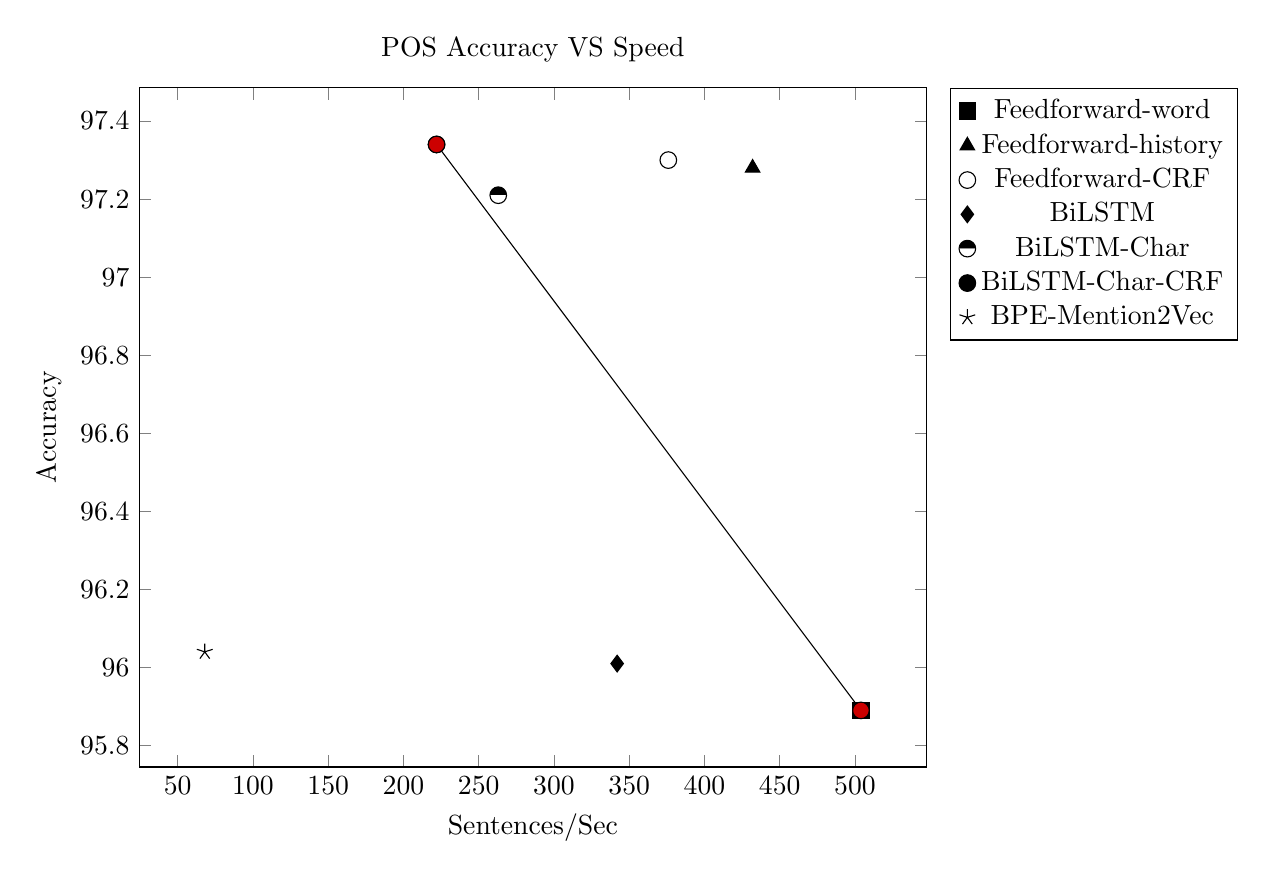
\begin{tikzpicture}
	\begin{axis}[%
	ylabel={Accuracy},
	xlabel={Sentences/Sec},
	scale only axis,
	mark size=3.0pt,
	title={POS Accuracy VS Speed},
	scatter/classes={%
		Feedforward-word={mark=square*},%
		Feedforward-history={mark=triangle*},%
		Feedforward-CRF={mark=o,draw=black},%
		BiLSTM={mark=diamond*},%
		BiLSTM-Char={mark=halfcircle*},%
		BiLSTM-Char-CRF={mark=otimes*},%
		BPE-Mention2Vec={mark=star}},%
	legend style={at={(1.03,1)},anchor=north west,draw=black,fill=white,align=left}]
	\addplot[scatter,only marks,%
		scatter src=explicit symbolic]%
	table[meta=label] {
    x     y      label
    504   95.89   Feedforward-word 
    432   97.28   Feedforward-history 
    376   97.30   Feedforward-CRF 
    342   96.01   BiLSTM 
    263   97.21   BiLSTM-Char
    222   97.34   BiLSTM-Char-CRF
    68    96.04   BPE-Mention2Vec
    };
    \addplot+ [color=black,mark=*]table {
    x     y      label
    504   95.89   Feedforward-word  
    222   97.34   BiLSTM-Char-CRF
    
    };
	\addlegendentry{Feedforward-word}
	\addlegendentry{Feedforward-history}
	\addlegendentry{Feedforward-CRF}
	\addlegendentry{BiLSTM}
	\addlegendentry{BiLSTM-Char}
	\addlegendentry{BiLSTM-Char-CRF}
	\addlegendentry{BPE-Mention2Vec}
	\end{axis}
\end{tikzpicture}
 \caption{Results of the POS system using different Neural Network Models}
  \label{fig:pos}
\end{figure}

\begin{figure}
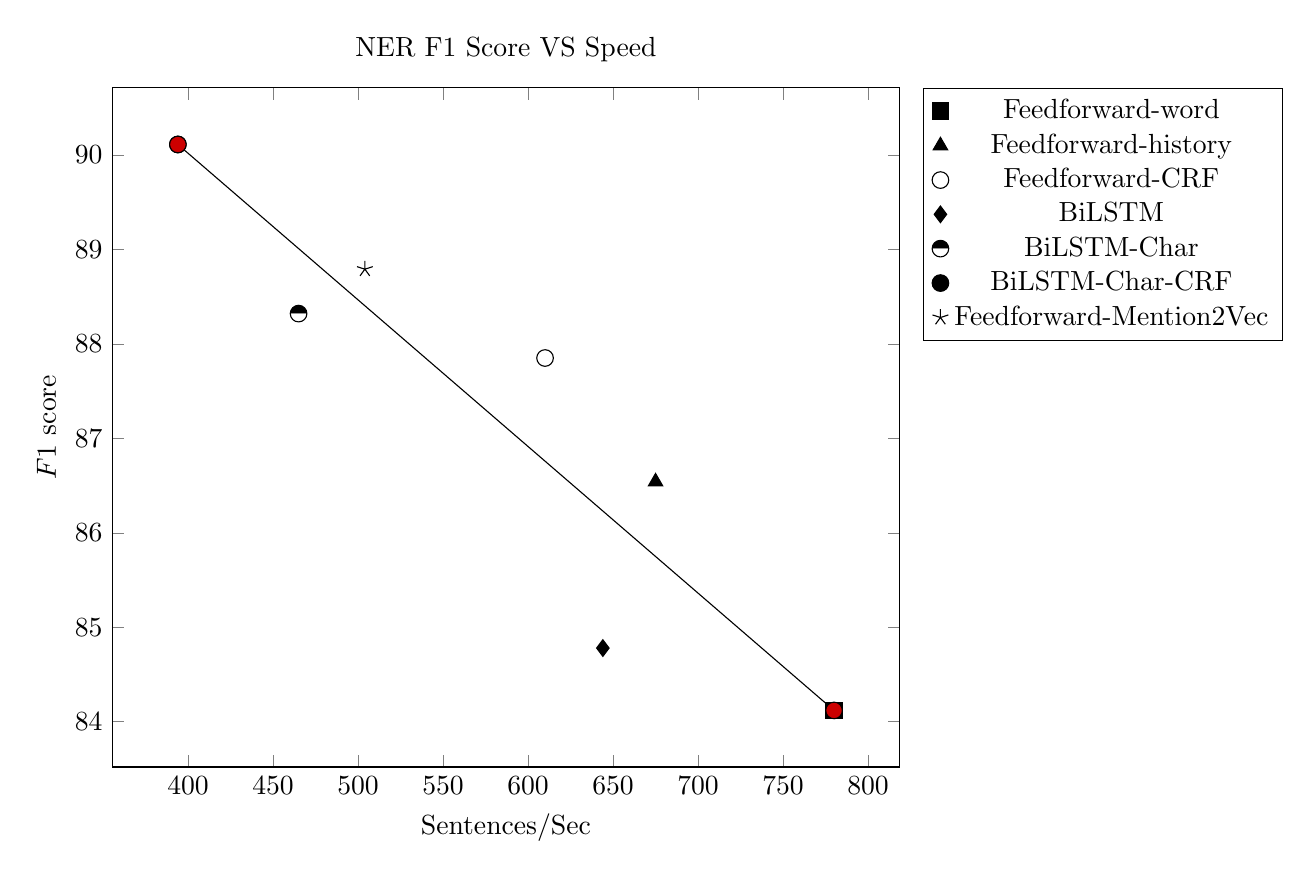
\begin{tikzpicture}
	\begin{axis}[%
	ylabel={$F1$ score},
	xlabel={Sentences/Sec},
	scale only axis,
	mark size=3.0pt,
	title={NER F1 Score VS Speed},
	scatter/classes={%
		Feedforward-word={mark=square*},%
		Feedforward-history={mark=triangle*},%
		Feedforward-CRF={mark=o,draw=black},%
		BiLSTM={mark=diamond*},%
		BiLSTM-Char={mark=halfcircle*},%
		BiLSTM-Char-CRF={mark=otimes*},%
		Feedforward-Mention2Vec={mark=star}},%
	legend style={at={(1.03,1)},anchor=north west,draw=black,fill=white,align=left}]
	\addplot[scatter,only marks,%
		scatter src=explicit symbolic]%
	table[meta=label] {
    x     y      label
    780   84.12   Feedforward-word 
    675   86.54   Feedforward-history 
    610   87.85   Feedforward-CRF 
    644   84.78   BiLSTM 
    465   88.32   BiLSTM-Char
    394   90.11   BiLSTM-Char-CRF
    504   88.79   Feedforward-Mention2Vec
	};
	\addplot+ [color=black,mark=*]table {
    x     y      label
    780   84.12   Feedforward-word 
    394   90.11   BiLSTM-Char-CRF
    
    };
	\addlegendentry{Feedforward-word}
	\addlegendentry{Feedforward-history}
	\addlegendentry{Feedforward-CRF}
	\addlegendentry{BiLSTM}
	\addlegendentry{BiLSTM-Char}
	\addlegendentry{BiLSTM-Char-CRF}
	\addlegendentry{Feedforward-Mention2Vec}
	\end{axis}
\end{tikzpicture}
 \caption{Results of the NER system using different Neural Network Models}
  \label{fig:ner}
\end{figure}

\chapter{Conclusions}

This thesis presents and compares different Neural Network models for sequence tagging. Our experiment result shows that simple Feedforward networks can achieve competitively results while being significantly faster than the recurrent BiLSTM models. Our experiments also demonstrate that the multitask Mention2Vec model performs well on the NER task.


%   BACK MATTER  %%%%%%%%%%%%%%%%%%%%%%%%%%%%%%%%%%%%%%%%%%%%%%%%%%%%%%%%%%%%%%
%
%   References and appendices. Appendices come after the bibliography and
%   should be in the order that they are referred to in the text.
%
%   If you include figures, etc. in an appendix, be sure to use
%
%       \caption[]{...}
%
%   to make sure they are not listed in the List of Figures.
%

%\backmatter%
\cleardoublepage
\phantomsection
\addtoToC{Bibliography}
%\bibliographystyle{apacite}
\bibliographystyle{apalike}
\bibliography{references}
	

%\begin{appendices} % optional
%	\chapter{Code}
%\end{appendices}
\end{document}
